\subsection{Ontology Engineering: the Design Process}
\label{sec:design-process}
\slidesrc{Ontology development: 2--60}

\textbf{Ontology engineering} is the discipline of building ontologies in a systematic
way, as software engineering is for programs. The slides include material by Valentina
Tamma, A.\ Gómez-Pérez, N.\ Noy, D.\ McGuinness, E.\ Kendal, A.\ Rector and O.\ Corcho.

% ---------------------------------------------------------------------------
\subsubsection{Many methodologies, one winner}
\slidesrc{Ontology development: 4--15}

Many methodologies have been proposed. The slides show the first page of several of
them, just to give an idea of how many there are:
\begin{itemize}[nosep]
  \item \emph{Ontology Engineering Methodologies} (Sure, Tempich, Vrandečić) and the
        \emph{Ontology Engineering Methodology} of Sure, Staab and Studer
        (On-To-Knowledge), focused on knowledge management in companies;
  \item \emph{HCOME}, Human-Centered Ontology Engineering (Kotis, Vouros, 2006): the
        ontology is developed collaboratively by communities of knowledge workers;
  \item \emph{DILIGENT} (Pinto, Staab, Tempich): for distributed, loosely controlled and
        evolving ontologies;
  \item the \emph{NeOn} methodology (Suárez-Figueroa, Gómez-Pérez, Fernández-López): no
        rigid workflow, nine scenarios (pathways) for building networks of ontologies;
  \item \emph{DOGMA} (Spyns, Tang, Meersman, STAR Lab, 2008);
  \item \emph{RapidOWL} (Auer): an \emph{agile} methodology, inspired by eXtreme
        Programming and wikis;
  \item the \emph{SWO project} (Copeland et al.): agile ontology engineering in
        community-driven ontologies;
  \item a literature review comparing them (Iqbal et al., 2013), which concludes that no
        methodology is completely mature.
\end{itemize}

``\ldots but for me the winner is'' (the lecturer's choice): Natalya F.\ Noy and
Deborah L.\ McGuinness, \textbf{Ontology Development 101: A Guide to Creating Your First
Ontology} (Stanford, 2001), already introduced in Section~\ref{sec:building-ontologies}.
It is one of the oldest and simplest methodologies, but still a good, flexible one
(cited by more than 9\,500 papers).

% ---------------------------------------------------------------------------
\subsubsection{The ontology design process}
\slidesrc{Ontology development: 16--18}

The design process has eight steps. They can be drawn as a straight pipeline, but in
reality the process is a \textbf{cycle}: after adding instances we discover problems and
go back to the requirements.

\begin{center}
\begin{tikzpicture}[st/.style={draw=nbblue, fill=nbblue!8, rounded corners=3pt,
    font=\footnotesize, align=center, text width=2.1cm, minimum height=0.85cm},
    arr/.style={-{Stealth}, thick, nbgray}]
  \foreach \t [count=\i from 0] in {Requirement and domain analysis, Determine scope,
      Consider reuse, Enumerate terms, Define classes, Define properties,
      Define constraints, Add instances}
     \node[st] (s\i) at ({90-\i*45}:3.2) {\t};
  \foreach \i [evaluate=\i as \j using {int(mod(\i+1,8))}] in {0,...,7}
     \draw[arr] (s\i) to[bend left=12] (s\j);
  \node[font=\small\itshape, text=nbgray, align=center] at (0,0) {iterate:\\ the design\\ is never
       final};
\end{tikzpicture}
\captionof{figure}{The ontology design process: eight steps, repeated in a cycle.}
\label{fig:design-cycle}
\end{center}

Compared with the seven steps of Section~\ref{sec:building-ontologies}, there is an
extra first step (requirement analysis) and the ``facets'' step is called
\emph{define constraints}. We now go through the steps on a running example.

% ---------------------------------------------------------------------------
\subsubsection{Steps 1--2: requirements and scope}
\slidesrc{Ontology development: 19--24}

\paragraph{Requirement analysis.}
As in any software engineering design, analysing the requirements, the domain and the
use cases is a critical stage: it grounds the work and lets the engineers set
priorities. It must make explicit:
\begin{itemize}[nosep]
  \item the nature of the knowledge and the \textbf{questions} (\emph{competency
        questions}) that the ontology, through a reasoner, must answer. This drives the
        scope, the design and the architecture;
  \item architectural issues.
\end{itemize}

\textbf{Application requirements} are found by:
\begin{itemize}[nosep]
  \item identifying any \textbf{controlled vocabulary} already used by the application;
  \item identifying \textbf{hierarchical (taxonomic) structures} intrinsic to the
        domain, which can be used for \emph{query expansion}: a query for
        \emph{vegetarian pizza} should also return margherita, funghi, grilled vegetables
        pizza;
  \item analysing \textbf{structured queries} and the knowledge they require;
  \item deciding the \textbf{expressive power} needed: efficient inference requires
        limited expressivity, more expressivity requires expensive (or resource-bounded)
        computation;
  \item ad-hoc reasoning for particular needs: temporal relations, geospatial reasoning,
        processes, conditional operations;
  \item computational tractability;
  \item need for explanations, traces, provenance (where a piece of knowledge comes
        from).
\end{itemize}

\textbf{Domain requirements} to take into account:
\begin{itemize}[nosep]
  \item heterogeneity, distribution and autonomy (e.g.\ applications made of software
        agents);
  \item \textbf{open vs.\ closed world}: does lack of information imply negative
        information? (see below);
  \item static vs.\ dynamic ontology processes (evolution, alignment);
  \item limited or incomplete knowledge; knowledge evolving over time;
  \item analysis and consistency checking of the instance data.
\end{itemize}
Use case analysis should clarify which \textbf{information} is likely to be available,
which \textbf{questions} are likely to be asked, and the \textbf{types and roles of
users}.

\paragraph{Determine the scope.}
Straightforward questions: what is the ontology going to be used for? How will the
software ultimately use it? What should the ontology be aware of, i.e.\ what is the
scope of the knowledge it must contain?

\begin{nbdef}{Competency questions}
\textbf{Competency questions} are questions, in natural language, that the ontology
must be able to answer. They define the scope (anything not needed to answer them can be
left out) and later serve as a test: if the ontology cannot answer them, it is not
finished.
\end{nbdef}

\begin{nbexample}{competency questions from the slides}
\begin{itemize}[nosep]
  \item Which investigations were done with a high-fat-diet study?
  \item Which study employs microarray in combination with metabolomics technologies?
  \item List those studies in which the fasting phase had as duration one day.
  \item What is a vegetarian pizza?
  \item What type of wine can accompany seafood?
\end{itemize}
The first three come from a biology ontology, the last two from the classic pizza and
wine examples. Each one names classes (study, technology, pizza, wine), properties
(duration, accompanies) and the kind of answer expected (a list of instances, a
definition, a class).
\end{nbexample}

% ---------------------------------------------------------------------------
\subsubsection{Step 3: consider reuse}
\slidesrc{Ontology development: 25--28}

We rarely have to start from scratch: there is almost always an ontology from a third
party that is at least a useful starting point. Reuse allows us
\begin{itemize}[nosep]
  \item to save effort;
  \item to interact with the tools that use other ontologies;
  \item to use ontologies already \emph{validated} through use in applications.
\end{itemize}
Standard vocabularies exist for most domains, and many overlap: we identify the set most
relevant to our problem. A \textbf{component-based approach based on modules} helps with
overlapping domains: we reuse an ontology module as we reuse a software module. Initial
brainstorming with domain experts can be very productive; refinement and iteration then
bring the ontology to the level required by the application.

What to reuse:
\begin{center}
\small
\begin{tabularx}{\linewidth}{@{}l X@{}}
\toprule
\textbf{kind} & \textbf{examples} \\
\midrule
ontology libraries & DAML ontology library, W3C ``Good Ontologies'' list, ontologies
  listed by Wikipedia, Protégé ontology library \\
upper ontologies & IEEE Standard Upper Ontology, Cyc \\
general ontologies & DMOZ (a Web directory), WordNet \\
domain-specific ontologies & UMLS Semantic Net (medicine), GO, the Gene Ontology
  (biology) \\
\bottomrule
\end{tabularx}
\end{center}
An \textbf{upper ontology} describes very general concepts (object, event, process,
time, space) shared by all domains; a \textbf{domain ontology} describes one domain.

% ---------------------------------------------------------------------------
\subsubsection{Step 4: enumerate terms}
\slidesrc{Ontology development: 29--31}

Write down, in an unstructured list, all the relevant terms expected to appear in the
ontology:
\begin{itemize}[nosep]
  \item \textbf{nouns} form the basis for \textbf{class} names;
  \item \textbf{verbs} (or verb phrases) form the basis for \textbf{property} names.
\end{itemize}
\textbf{Card sorting} is often the best way: write each concept on a card, organise the
cards into piles, link the piles together, and do it again, and again. It works best in
a small group.

\begin{nbexample}{animals \& plants: the raw list of terms}
Dog, Cat, Cow, Person, Tree, Grass, Herbivore, Male, Female, Dangerous, Pet, Domestic
animal, Farm animal, Draft animal, Food animal, Fish, Carp, Goldfish, Carnivore, Plant,
Animal, Fur, Child, Parent, Mother, Father.

At this stage the list is a mess on purpose: it mixes kinds of things (Dog, Plant),
properties (Dangerous, Male), roles (Pet, Parent) and parts (Fur). Sorting them out is
the job of the next step.
\end{nbexample}

% ---------------------------------------------------------------------------
\subsubsection{Step 5: define classes and their taxonomy}
\slidesrc{Ontology development: 32--43}

\begin{nbdef}{Class and instance}
A \textbf{class} is a concept in the domain (Animal; or a class of roles, like Father,
Mother): a collection of elements with similar properties. A class can state
\emph{necessary conditions for membership} (type of food, dwelling). An
\textbf{instance} of a class is a particular element: a particular farm animal, a
particular person, \emph{Tweety the penguin}.
\end{nbdef}

\paragraph{Organise the concepts.}
Take a group of things and ask what they have in common, then which other ``siblings''
there might be:
\begin{itemize}[nosep]
  \item Plant, Animal $\to$ \emph{Living thing} (we might add Bacteria and Fungi, but not
        now);
  \item Cat, Dog, Cow, Person $\to$ \emph{Mammal} (others: Goat, Sheep, Horse, Rabbit,
        \ldots);
  \item Cow, Goat, Sheep, Horse $\to$ \emph{Hoofed animal} (``Ungulate''). What others
        are there? Do they divide among themselves?
  \item Wild, Domestic $\to$ \emph{Domestication}. What other states are there?
        ``Feral'' (a domestic animal returned to the wild).
\end{itemize}

\paragraph{Choose some main axes.}
Add abstractions where needed (e.g.\ ``Living thing''); identify \textbf{relations}
(\emph{eats}, \emph{owns}, \emph{parent of}), which feed the next step; identify
\textbf{definable} things (child, parent, mother, father): things for which you can say
clearly what they mean in terms of other things. Make names explicit.

\paragraph{Self-standing entities and modifiers.}
\begin{itemize}[nosep]
  \item \textbf{Self-standing entities}: things that can exist on their own: people,
        animals, houses, actions, processes, \ldots\ Roughly the \emph{nouns}.
  \item \textbf{Modifiers}: things that modify (``inhere in'') other things. Roughly the
        \emph{adjectives} and \emph{adverbs}.
\end{itemize}

\begin{nbfact}{the method of the primitives}
Reorganise everything except the \emph{definable} things into \textbf{pure trees} (each
class has exactly one parent): these are the \textbf{primitives}. The definable things
are not placed in the tree by hand: they are \emph{defined} in terms of the primitives
(step~7), and the reasoner computes where they belong.
\end{nbfact}

\begin{center}
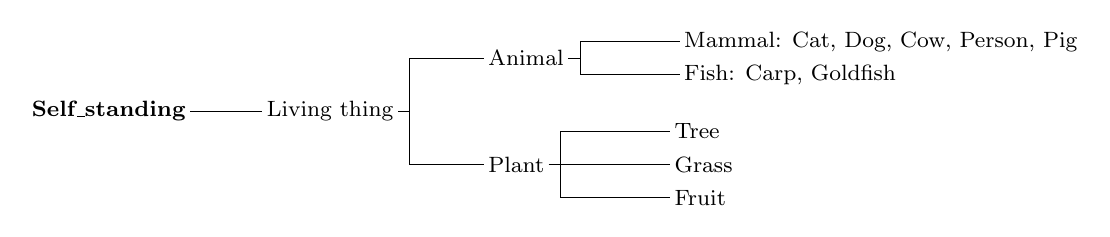
\begin{tikzpicture}[
    grow'=right, level distance=1.95cm, edge from parent path={(\tikzparentnode.east) -- ++(0.15,0) |- (\tikzchildnode.west)},
    every node/.style={font=\footnotesize, anchor=west, inner sep=1.5pt},
    level 1/.style={sibling distance=2.7cm},
    level 2/.style={sibling distance=1.35cm},
    level 3/.style={sibling distance=0.42cm}]
  \node[font=\footnotesize\bfseries] {Self\_standing}
    child {node {Living thing}
      child {node {Animal}
        child {node {Mammal: Cat, Dog, Cow, Person, Pig}}
        child {node {Fish: Carp, Goldfish}}}
      child {node {Plant}
        child {node {Tree}}
        child {node {Grass}}
        child {node {Fruit}}}};
\end{tikzpicture}

\medskip
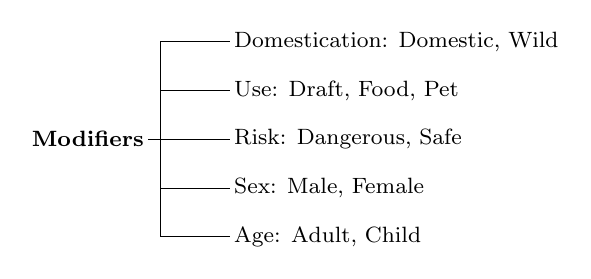
\begin{tikzpicture}[
    grow'=right, level distance=1.8cm, edge from parent path={(\tikzparentnode.east) -- ++(0.15,0) |- (\tikzchildnode.west)},
    every node/.style={font=\footnotesize, anchor=west, inner sep=1.5pt},
    level 1/.style={sibling distance=0.62cm}]
  \node[font=\footnotesize\bfseries] {Modifiers}
    child {node {Domestication: Domestic, Wild}}
    child {node {Use: Draft, Food, Pet}}
    child {node {Risk: Dangerous, Safe}}
    child {node {Sex: Male, Female}}
    child {node {Age: Adult, Child}};
\end{tikzpicture}
\hspace{0.1cm}
\begin{tabular}[b]{@{}l@{}}
\textbf{Definables}\\ Carnivore, Herbivore\\ Child, Parent\\ Mother, Father\\
Food animal, Draft animal\\[4pt]
\textbf{Relations}\\ eats, owns, parent-of, \ldots
\end{tabular}
\captionof{figure}{The animals \& plants terms reorganised: self-standing entities and
modifiers as pure trees (the primitives), plus the definables and the relations, kept
aside.}
\label{fig:animals-plants}
\end{center}

\begin{nbintuition}[why pure trees?]
\emph{Pet} looks like a subclass of \emph{Animal}, \emph{Dog} too; but a dog can be a
pet or not, and a pet can be a dog, a cat or a goldfish. If we put \emph{Pet} in the
same tree as \emph{Dog} we get multiple inheritance everywhere and the tree becomes a
tangle. Keeping ``what a thing is'' (Dog) separate from ``how it is used'' (Pet) and
``what state it is in'' (Domestic) keeps each tree simple. A class like \emph{Pet dog}
can then be \emph{defined} as Dog $\sqcap$ having use Pet, and the reasoner works out
that it is both a Dog and a Pet.
\end{nbintuition}

\textbf{Comments help to clarify}: when a class is used in a special way, add a comment,
e.g.\ on \emph{Living thing}: ``abstract ancestor concept including all living things;
restrict to plants and animals for now''.

\paragraph{Class inheritance.}
Classes are organised into \textbf{subclass--superclass} hierarchies (also called
generalisation--specialisation hierarchies). Two classes are in an ``is-a'' relation if every instance of the subclass
is an instance of the superclass. Classes can be seen as \textbf{sets}: a subclass is a
subset of its superclass. Examples: Mammal is a subclass of Animal; every penguin is a
bird (Tweety, an instance of Penguin, is also an instance of Bird); Draft animal is a
subclass of Animal.

\paragraph{Levels in the class hierarchy.}
Three modes of development:
\begin{itemize}[nosep]
  \item \textbf{top-down}: define the most general concepts first and then specialise
        them;
  \item \textbf{bottom-up}: define the most specific concepts first, then group them into
        more general classes;
  \item a \textbf{combination} (the typical choice): breadth at the top level and depth
        along a few branches to test the design.
\end{itemize}
\textbf{Class inheritance is transitive}: if A is a subclass of B and B a subclass of C,
then A is a subclass of C.

\begin{center}
\begin{tikzpicture}[w/.style={font=\small, anchor=west, inner sep=1pt}, y=0.48cm,
    br/.style={decorate, decoration={brace, amplitude=4pt}, thick}]
  \node[w] at (0,0) {Wine};
  \foreach \t/\y in {White wine/1, Rosé wine/2, Red wine/3}
     {\node[w, text=nbgreen!60!black] at (0.5,-\y) {\t}; \draw[nbgray] (0.2,-\y+0.6) |- (0.5,-\y);}
  \foreach \t/\y in {Beaujolais/4, Red Burgundy/5, Red Zinfandel/6, Red Bordeaux/7}
     {\node[w, text=nbblue] at (1.0,-\y) {\t}; \draw[nbgray] (0.7,-\y+0.6) |- (1.0,-\y);}
  \foreach \t/\y in {Médoc/8}
     {\node[w, text=nbteal] at (1.5,-\y) {\t}; \draw[nbgray] (1.2,-\y+0.6) |- (1.5,-\y);}
  \foreach \t/\y in {Pauillac/9, Margaux/10}
     {\node[w, text=nbteal] at (2.0,-\y) {\t}; \draw[nbgray] (1.7,-\y+0.6) |- (2.0,-\y);}
  \foreach \t/\y in {St.\ Émilion/11, Graves/12}
     {\node[w, text=nbteal] at (1.5,-\y) {\t}; \draw[nbgray] (1.2,-\y+0.6) |- (1.5,-\y);}
  \foreach \t/\y in {{Cabernet Franc, Cabernet Sauvignon, Pinot Noir, Chianti, \ldots}/13}
     {\node[w, text=nbblue] at (1.0,-\y) {\t}; \draw[nbgray] (0.7,-\y+0.6) |- (1.0,-\y);}
  \draw[br, nbgreen!60!black] (3.2,-0.7) -- (3.2,-3.3) node[midway, right=5pt, font=\small\bfseries] {top level};
  \draw[br, nbblue] (4.4,-3.7) -- (4.4,-7.3) node[midway, right=5pt, font=\small\bfseries] {middle level};
  \draw[br, nbteal] (4.4,-7.7) -- (4.4,-12.3) node[midway, right=5pt, font=\small\bfseries] {bottom level};
\end{tikzpicture}
\captionof{figure}{Levels in the class hierarchy of the wine ontology (redrawn and
simplified from a Protégé screenshot): general classes at the top, specific ones at the
bottom.}
\end{center}

% ---------------------------------------------------------------------------
\subsubsection{Step 6: define properties}
\slidesrc{Ontology development: 44--47}

This step is often interleaved with the previous one. \textbf{Properties} (called
\emph{roles} in description logics, \emph{slots} in frames) describe the attributes of
the members of a class.

\begin{nbfact}{properties are inherited}
The semantics of \emph{subClassOf} demands that whenever A is a subclass of B, every
property statement that holds for instances of B also applies to instances of A. So it
makes sense to attach a property to the \textbf{highest} class in the hierarchy to which
it applies (attach \emph{eats} to Animal, not separately to Cat, Dog, Cow, \ldots).
\end{nbfact}

Types of properties, on the wine example:
\begin{itemize}[nosep]
  \item \textbf{intrinsic} properties: flavour and colour of a wine (they belong to the
        thing itself);
  \item \textbf{extrinsic} properties: name and price of a wine (assigned from outside);
  \item \textbf{parts}: the ingredients of a dish;
  \item \textbf{relations to other objects}: the producer of a wine (a winery).
\end{itemize}
They are represented by two kinds of properties (Section~\ref{sec:ontology-languages}):
\begin{itemize}[nosep]
  \item \textbf{datatype properties}: simple values (strings, numbers): name, price;
  \item \textbf{object properties}: complex values, other objects: the producer is an
        instance of Winery.
\end{itemize}
In the animals example, the modifiers of Figure~\ref{fig:animals-plants} (domestication,
use, risk, sex, age) and the relations (eats, owns, parent-of) become properties.

% ---------------------------------------------------------------------------
\subsubsection{Step 7: define constraints}
\slidesrc{Ontology development: 48--56}

\paragraph{Domain and range.}
For each property, state the \textbf{domain} (the class of the things that can have it)
and the \textbf{range} (the class of its values):
\begin{center}
\small
\begin{tabularx}{\linewidth}{@{}>{\raggedright\arraybackslash}X l l l@{}}
\toprule
\textbf{statement} & \textbf{property} & \textbf{domain} & \textbf{range} \\
\midrule
Animal eats Living\_thing & eats & Animal & Living\_thing \\
Person owns Living\_thing except person & owns & Person & Living\_thing $\sqcap \neg$Person \\
Living\_thing parent\_of Living\_thing & parent\_of & Living\_thing & Living\_thing \\
\bottomrule
\end{tabularx}
\end{center}
If anything is used in a special way, add a text comment. E.g.\ on \emph{eats}:
``ignore the difference between parts of living things and living things; also things
derived from living things'' (strictly, a cow eats \emph{leaves}, not whole plants, and
we eat cheese, which is not a living thing).

\paragraph{Definable things.}
Paraphrase the definitions and formalise them in terms of the primitives, the relations
and other definables. Note any assumptions (as comments when implementing).

\begin{nbexample}{three definitions}
The slides write them in the Manchester syntax used by Protégé (\emph{and}, \emph{some},
\emph{only}); next to it the same in description-logic notation, where $\sqcap$ is
``and'', $\exists r.C$ is ``has some $r$-value in $C$'' and $\forall r.C$ is ``all
$r$-values are in $C$'':
\begin{center}
\small
\begin{tabularx}{\linewidth}{@{}>{\raggedright\arraybackslash}X l@{}}
\toprule
\textbf{in words} & \textbf{formal} \\
\midrule
A \emph{Parent} is an animal that is the parent of some other animal (ignore plants for
  now) & Parent $\equiv$ Animal $\sqcap\ \exists$parent\_of.Animal \\
A \emph{Herbivore} is an animal that eats only plants & Herbivore $\equiv$ Animal
  $\sqcap\ \forall$eats.Plant \\
An \emph{Omnivore} is an animal that eats both plants and animals & Omnivore $\equiv$
  Animal $\sqcap\ \exists$eats.Animal $\sqcap\ \exists$eats.Plant \\
\bottomrule
\end{tabularx}
\end{center}
\end{nbexample}

\begin{nbwarning}[``only'' does not mean ``some'']
$\forall$eats.Plant (``eats \emph{only} plants'') is also true of something that eats
\emph{nothing}: all the (zero) things it eats are plants. That is why the slides add
``NB: all animals eat some living thing'': with that axiom, an animal that eats only
plants really eats some plant. Mixing up \emph{some} ($\exists$) and \emph{only}
($\forall$) is the most common modelling error in OWL.
\end{nbwarning}

\paragraph{Fill in properties at the class level.}
What can we say about \emph{all} members of a class? All cows eat some plants; all cats
eat some animals; all pigs eat some animals and eat some plants. In Protégé this can be
done with a ``property matrix'' (one row per class, one column per property: Cat eats
Animal, Dog eats Animal, Cow eats Grass and Leafy\_plant, Person eats Animal and Plant).

\paragraph{Check with the classifier: the closure axiom.}
A \textbf{classifier} (reasoner) computes the hierarchy of the defined classes. We expect
\emph{Cow} to be classified as a \emph{Herbivore}. It is not. Why?

\begin{nbexample}{why cows are not herbivores (yet)}
What we have said: cows are animals and, among other things, eat some grass and eat some
leafy plants:
\[
  \text{Cow} \sqsubseteq \text{Mammal} \sqcap \exists\text{eats.Grass} \sqcap
  \exists\text{eats.Leafy\_plant}.
\]
Nothing here says that cows eat \emph{only} plants: a cow could also eat some animal,
and the reasoner must allow that. What we need to say: cows eat some plants
\textbf{and eat only plants}. We add the \textbf{closure axiom}
\[
  \text{Cow} \sqsubseteq \forall\text{eats.}(\text{Grass} \sqcup \text{Leafy\_plant}),
\]
which ``closes'' the list of things cows eat. Now every cow is an Animal that eats only
plants, so the reasoner classifies Cow under Herbivore.
\end{nbexample}

\begin{nbdef}{Open vs.\ closed world reasoning}
\begin{itemize}[nosep]
  \item \textbf{Open world} reasoning: \emph{negation as contradiction}. Anything might
        be true unless it can be proven false. We reason about \emph{any} world
        consistent with what we know.
  \item \textbf{Closed world} reasoning: \emph{negation as failure}. Anything that cannot
        be found is false. We reason about \emph{this} world, the one in the database.
\end{itemize}
OWL ontologies use the open world assumption: \textbf{ontologies are not databases}
(Section~\ref{sec:what-is-an-ontology}).
\end{nbdef}

\begin{nbintuition}[the closure axiom and the open world]
In a database, if the table of what cows eat lists only grass and leafy plants, then cows
eat nothing else: missing rows are false (closed world). In an ontology, missing
information is just \emph{unknown} (open world): ``cows eat grass'' leaves open that they
also eat fish. The closure axiom is how we tell an open-world reasoner ``and that is
all''.
\end{nbintuition}

% ---------------------------------------------------------------------------
\subsubsection{Step 8: create instances}
\slidesrc{Ontology development: 57--60}

To create an instance of a class: the class becomes the \textbf{direct type} of the
instance, and every superclass of the direct type is also a type of the instance (Tweety
is a Penguin, hence a Bird, hence an Animal). Then assign the slot (property) values;
they must conform to the facet constraints, and knowledge-acquisition tools often check
this.

Filling the ontology with instances is a \textbf{separate step}, and the number of
instances is much larger than the number of classes. So \textbf{populating} an ontology
is usually not done by hand: instances are retrieved from legacy data sources
(databases) or \textbf{extracted automatically from a text corpus}: this is
\emph{ontology population}, part of ontology learning (Section~\ref{sec:ontology-learning}).

\begin{nbsummary}[the design process]
\begin{itemize}[nosep]
  \item Many methodologies (On-To-Knowledge, HCOME, DILIGENT, NeOn, DOGMA, RapidOWL,
        \ldots); the lecturer's choice: Noy \& McGuinness, \emph{Ontology Development
        101}.
  \item Cycle of 8 steps: requirement and domain analysis $\to$ scope $\to$ reuse $\to$
        enumerate terms $\to$ classes $\to$ properties $\to$ constraints $\to$
        instances, and again.
  \item Competency questions define the scope and test the ontology.
  \item Reuse: libraries, upper ontologies (SUO, Cyc), general (WordNet), domain (GO,
        UMLS).
  \item Terms: nouns $\to$ classes, verbs $\to$ properties; card sorting.
  \item Classes: self-standing entities and modifiers as pure trees (primitives);
        definables defined by axioms; inheritance is transitive; top-down, bottom-up or
        combined.
  \item Properties: intrinsic, extrinsic, parts, relations; datatype vs.\ object; attach
        to the highest class.
  \item Constraints: domain and range; definitions with \emph{some} ($\exists$) and
        \emph{only} ($\forall$); closure axioms; open world (ontology) vs.\ closed world
        (database).
  \item Instances: many, populated automatically from databases or text.
\end{itemize}
\end{nbsummary}
